\begin{savequote}[8cm]
%If you wish to understand the Universe, think of energy, frequency and vibration.
%  \qauthor{--- Nikola Tesla}
I'm pickin' up good vibrations.
 \qauthor{--- The Beach Boys, \textit{Good Vibrations}}
\end{savequote}

\chapter{\label{ch:5-epcoupling}Results II: Electron-phonon and phonon-phonon coupling}
% see ziman electrons and phonons?
% https://journals.aps.org/rmp/pdf/10.1103/RevModPhys.89.015003
\section{Introduction} \label{ch5:introduction}

% simplest approximation is that there is no coupling. But then mobility too large. In reality scattering (see previous chapter)
%include v. brief overview of what each is and explain that it is linked to non-radiative recombination and other important processes, thermal transport.
In the simplest approximation of a semiconductor, a single electron in a perfect lattice at zero kelvin, electrons do not scatter and have infinite mobility. In the next best approximation, we introduce harmonic phonons. The electrons scatter from the phonons and the electron mobility becomes finite. This electron-phonon interaction underpins many phenomena in condensed matter physics and materials science including carrier mobility (as explored briefly in the previous chapter, Section \ref{}), polaron formation (Section \ref{}), hot carrier thermalisation (Section \ref{}) and carrier capture (Section \ref{}). Still, in the harmonic phonon approximation, the phonons do not interact with one another - they have an infinite lifetime. To calculate thermal conductivity or understand how a polaron cools to equilibrium (Section \ref{}) we need to consider anharmonic phonon-phonon interactions. Some processes involve electron-phonon and phonon-phonon interactions; for example during non-radiative recombination carrier capture and lattice relaxation proceed via the electron-phonon and phonon-phonon interactions respectively. 

This chapter begins with an introduction to electron-phonon coupling, with coupling to acoustic and optical phonon modes considered. This extends the discussion in Section \ref{ch2epcoupling} and references the broader underlying theory. Phonon-phonon coupling is discussed in Sections \ref{ch2anharmonic} and \ref{anharmonicapprox}; how this relates to ``hot-carrier cooling" is introduced below.

% Can measure a temperature dependance in the electronic structure:, Peaks shift, Peaks broaden (shorter electron lifetime), There is a direct and indirect (through the change in volume) contribution to dE/DT. , For direct: See AHC theory., For the indirect what we are asking is the effect of thermal expansion. See monserrat work or Bi2Se3 where it is not negligible. For Si the expansion is negligible (Xavier Gonze)

\subsection{Electron-phonon coupling}
In equation \ref{} we consider a system under the Born-Oppenheimer approximation, where the electronic and vibrational substates are decoupled; $ $.%the full wavefunction product of ht other two.
To consider the effect of electron-phonon interactions we must consider a hamiltonian describing a coupled system and include a previously ignored term to the system Hamiltonian:\cite{Giustino2016}
\begin{equation} \label{HamiltonianEP}
    \hat{H} = \sum_{nk}\epsilon_{nk}\hat{c}^{\dagger}_{nk}\hat{c}_{nk} + \sum_{qv}\hbar\omega_{qv}(\hat{a}^{\dagger}_{qv}\hat{a}_{qv}+\frac{1}{2})+N_p\sum...
\end{equation}
The first two terms describe the separate electron and phonon sub-systems, as seen in Section \ref{}. The third term describes the electron-phonon interaction. The electron has an energy eigenvalue $\epsilon$, determined by the crystal momentum $k$ and band $n$. This electron is interacting with a phonon of vibrational frequency $\omega$  , determined by crystal momentum $q$ and branch $v$. The matrix element $g$ determines the strength of the coupling. 

Unfortunately Equation \ref{HamiltonianEP} does not tell us how to calculate the coupling term $g$. The first expression of $g$ was derived by Bloch in 1929:
%\begin{equation}
%%    
    
%\end{equation}
where $V_0$ is the effective potential experienced by the electrons in the crystal.

\textbf{Acoustic deformation potential scattering}\\
 In 1950 Bardeen and Shockley introduced the `deformation potential' method \cite{}, which gives an approximation to $V_0$ for semiconductors where the dominant electron-phonon scattering mechanisms involve long wavelength acoustic phonons.\cite{Giustino2016} In this approach $g$ is given by:
\begin{equation} \label{couplingterm}  % edit this just for V_0
   q_{mnv}(k,q) = \i\left(\frac{\hbar}{2N_pM_k\omega_{qv}}\right)^{\frac{1}{2}}q\cdot e_{kv}(q) \Omega\frac{\partial\epsilon_{nk}}{\partial\Omega},
\end{equation}
where $N_p$ the number of cells in the supercell, $M_k$ is the mass of the $k^{\textrm{th}}$ supercell and $\textbf{e}_\textrm{{kv}}$ is the polarization of the phonon. 

The deformation potential $\Omega\frac{\partial\epsilon_{nk}}{\partial\Omega}$ in Equation \ref{couplingterm} can be determined empirically or calculated from first principles using DFT. 
Density-functional perturbation theory (DFPT) is a common method used to calculate  electron-phonon  coupling. However DFPT assumes a small harmonic response for the perturbative treatment to be correct and for anharmonic phonon modes, where the range of motion is large, this assumption does not hold.
Instead, the `frozen phonon' method can be used: here the energy of the valence and conduction bands are tracked as the crystal lattice is distorted along a single phonon mode. 
%The coupling term $g$ is given by 
%\begin{equation}
%    q_{mnv}(k,q) = \langleu_{mK=q}|\Delta_{qv}v^{KS}|u_{nk}\rangle_{uc}
%\end{equation}

\textbf{Frolich interactions}\\
For Frolich interactions, the electrons are affected by the electric field generated by longitudinal optical (LO) phonons.
This interaction is available only in ionic crystals, where atomic displacements generate long-range electric fields. In the Frolich model a single electron interacts with the polarization field of an ionic lattice.\cite{Giustino2016}
In this model the effective potential is replaced with
\begin{equation}
    V_0 = \left[\frac{e^2M_k\omega^2_{qv}}{\epsilon_0\Omega}\left(\frac{1}{\epsilon^{\infty}}-\frac{1}{\epsilon^0}\right)\right]^{\frac{1}{2}}\frac{1}{|q|^2}
\end{equation}
where $\epsilon_0$,$\epsilon^0$ and $\epsilon^{\infty}$ is the vacuumn static relative and high-frequency relative permittivities respectively.

MAPI is a soft material, with structural distortions and dynamic disorder at room temperature, so electron-phonon interactions are expected to be significant 
Furthermore, long carrier lengths but modest mobilities in MAPI point to strong electron-phonon interactions.\cite{} 
% https://pubs.acs.org/doi/pdf/10.1021/acs.jpclett.5b02390 
Photoluminescence studies of FAPI suggest that acoustic deformation potential scattering makes only a minor contribution to electron-phonon interactions at room temperature, \cite() %  Electron-Phonon Coupling in Hybrid Lead Halide Perovskites.Nat. Commun.2016,7, 11755
whilst electron-phonon coupling is reduced below the temperature correponding to the relevant LO phonon for Frolich coupling. This suggests that Frolich interactions dominate, and is supported by a theoretical calculation which predicts a LO-phonon limited mobility in line with experiment.\cite{Jarv}

% Robert Lobronvnic Optical phonon modes hbarw are occupied at kT @ room temperature: RARE
\subsection{Hot carrier cooling in hybrid halide perovskites}

Halide perovskites display unusual cooling kinetics for electrons photo-excited above the bandgap.% 10.1021/jacs.6b088804 doi:10.1038/ncomms14350  DOI: 10.1038/ncomms14120 doi:10.1038/nphoton.2015.213
The cooling of these ``hot" electrons is slower than that observed in other semiconductors and this has been attributed to a ``hot phonon bottleneck".\cite{} % doi:10.1038/ncomms14350  DOI: 10.1038/ncomms14120 doi:10.1038/nphoton.2015.213
Hot carrier cooling in the hybrid perovskites can be split into three stages: i) transfer of energy from the electron to optical phonons (via the electron-phonon Frolich interaction); ii) optical phonon decay into acoustic phonons (phonon-phonon interaction); iii) acoustic phonon propagation (phonon-phonon interaction).
The phonon bottleneck results from the equilibriation of hot carriers with a non-equilibrium phonon population;
Frolich interactions strongly couple the hot electrons to longitudinal optical (LO) phonons, but the LO phonons are not able to dissipate their heat. 
This could be due to poor coupling between the optical and acoustic phonon modes, or because acoustic phonon mode propagation is blocked and the phonon modes re-heat carriers.
In either case, two timescales appear experimentally; fast initial thermalisation with optical phonons via the Frolich interaction, followed by slower cooling to equilibrium with the extended bulk solid (Figure \ref{}).
The phonon bottleneck appears above a particular carrier density. Transient absorption spectroscopy identifies  $10^18\,\textrm{cm}^{-3}$.doi:10.1038/nphoton.2015.213 as the critical carrier density for MAPI.

\begin{figure}[h!]
\centering
  \includegraphics[width=0.7\columnwidth]{figures/ch5/f1.pdf}
  \caption[Hot carrier cooling model]{Figure prepared by Aron Walsh.}
\label{cooling_schematic}
\end{figure}

%    Cooling is ten times slower in FAPI than in Caesium-based. Postulate that up-conversion of low-energy phonons is responsible, and this is possible dues to overlapping phonon branches of organic cations. Also due to blocking of phonon propagation with ultralow thermal conductivity. Two stages in cooling are identified; the first is independant of fluence whlst the second is not. First is attributed to Frolich phonon emission (electron and LO phonon coupling). Similar between Cs and organic as the electronic band structure near the band edge is dominated by the inorganic PbI framework. Second stage appears when sufficient fluence is used. Higher fluence means longer cooling lifetime.
 %   MAPI has a poor hot carrier response cmopared to FAPI. .MAPI is found to have much faster cooling time than FAPI. This is explained by lattice defects. Faster carrier relaxation indicates a large number of above band gap defects which provide relaxation pathways for hot carriers. A second power dependant hot phonon bottleneck effect is found.
% Carrier thermalisation --> LO emission ---> acoustic phonon decay ---> local lattice heating ---> acoustic phonon propagation and the heat is dispersed. So three stages: (1) carrier-phonon (Frolich interaction) (2) Optical phonon decay to acoustic phonons (3) acoustic phonon propagation.
 % Things that can increase the overall cooling period are (1) thermal isolation between optical phonon and carriers (achieved through large polaron effect). Ruled out here as power independant second stage but not first. (2) reducing the phonon dos (opening the phonon bandgap using large atomic mass differences, gap twice the highest acoustic phonon). Not seen here. (3) acoustic up-conversion to optical phonons (local lattice heat doesn't dissipate to surroundings but reheats carriers)
   % Optical phonon modes in hybrids show a relatively flat band compared with inorganic case - non-propagating vibrations on the organic cation. Cascade decay of LO phonons may slow cooling.
 %   Hybrid phonon modes which are covibrations between organic and inorganic lattice. Excited by phonon-phonon scattering events. Show littel dispersion and have good overlap with coustic branches. So acoustic phonons scatter to optical states. Anharmonic phonon-phonon scattering, low thermal conductivity, means that propagation blocked and increase probabilty of up-transition.


%\begin{figure}[h!]
%\centering
%  \includegraphics[width=0.7\columnwidth]{C05/figs/f1.pdf}
%  \caption{Reproduced from reference \cite{Whalley2017a}.}
%  \label{cooling_schematic}
%\end{figure}
%\section{Summary}

% what is happening in this chapter: calculated for MAPI.
% Modes are the soft modes: Anharmonic soft tilting modes are characteristic of the perovskite material family. For cubic perovskite with a unit cell of The tilting corresponds to opposite tilting in neighbour cell, so happens at M (0.5,0,0) amd R (0.5,0.5,0). Hybrid halide perovskites have double-well potentials associated with octahedral tilting of the inorganic lattice. These are located at the $M$ and $R$ point in the brillouin zone.
%We use a `mode mapping' approach to distort the structure along the $M$ and $R$ eigenvectors and track the change in bandgap as a function of the normal mode coordinate $Q$ (which corresponds to the amplitude of the phonon mode).


\section{Methods}
\subsection{Calculation procedures for bandgap deformation potential}

The bandgap deformation potentials were calculated using the frozen phonon method.
\ce{Phonopy}\cite{} was used to calculate the harmonic phonon eigenvalues and eigenvectors. $2\,\times2\,\times2$ supercell expansions and displacement steps of 0.01 were used to evaluate the second-order and force-constant matrices using the finite-displacement method. ModeMap scripts available online\cite{} were used to generate a sequence of structures along the phonon eigenvectors at the $M$ and $R$ points in reciprocal space. 

The deformation potentials were calculated by following the phonon mode vectors and mapping the change in band gap as a function of normal mode coordinate $Q$.
Bandgaps were computed within the Kohn-Sham density-functional theory (DFT) formalism as implemented in the \textsc{VASP} code\cite{Kresse1996a}.
The valence wavefunctions were expanded in a plane-wave basis set with a 700 eV cut-off and the exchange and correlation interactions between electrons were modelled using the PBEsol exchange-correlation functional\cite{Perdew2008a} ($Q$ from 0 to 150 amu$^{\frac{1}{2}}$ \AA) and a screened hybrid functional (HSE06)\cite{Heyd2004a,Heyd2005a} ($Q$ from 0 to 69 amu$^{\frac{1}{2}}$ \AA).
Scalar-relativistic corrections were used for the core electrons within the projector augmented-wave (PAW) formalism,\cite{Blochl1994} with the outermost s and p electrons of C, N and I, and the outermost s, p and d electrons of Pb, being treated as valence. 
The PAW projection was applied in reciprocal space (\textsc{LREAL = .FALSE.} in \textsc{VASP}).
Spin-orbit coupling, which strongly affects the unoccupied conduction band, was considered for the PBEsol functional.
A Monkhorst-Pack \textit{k}-point grid, with a $\Gamma$-centered $6 \times 6 \times 6$ grid, was used to integrate the electronic Brillouin zone.
A total-energy convergence criterion of $10^{-8}$ eV during the electronic minimisation was found to be necessary to remove noise in the absolute electronic eigenvalues.
A least-squares polynomial fit using the \textsc{Python} library \textsc{Numpy} was applied to the symmetrised data.

% cite Jarvist work
\subsection{Classical model for hot carrier cooling}
The hot carrier cooling rate was modelled classically. The polaron was considered as a hot-sphere in a continuum of ambrient-temperature material. This reduces the problem to one-dimension, where the exponent is weighted by the $r^2$ increasing shell of available states over the surface of the sphere. 
The initial “top hat” heat distribution was convolved with a Gaussian kernel to give an analytical expression for the evolution of hot carrier energy with time.
The rate of cooling was determined by the diffusivity $D$:
\begin{equation}
    D = \frac{\kappa}{\rho c_p}
\end{equation}
where $\kappa$ is the thermal conductivity, $\rho$ is the density, and $c_p$ is the specific heat capacity. A derivation of the diffusion equation for a hot sphere is given in the Appendix (\ref{app:2-diffusion}).

\section{Results}
\subsection{Anharmonic bandgap deformation potential}
The change in band gap as a function of normal mode coordinate $Q$ is plotted in Figure \ref{ch5figs1}. Distortions are along soft acoustic phonon modes at the $M$ and $R$ $q$-points, which correspond to in-phase and out-of-phase tilting of the inorganic octahedra respectively.
We find that the bandgap $E_g(Q)$ is well described as quadratic over small $Q$, but that a bi-quadratic term is required to reproduce the correct behaviour at large $Q$ (Table \ref{ch5rsstable}). 
The significance of the bi-quadratic term is apparent when calculating the average band gap as a function of temperature (Section \ref{ch5coupling}; the quadratic fit leads to a predicted band gap twice as large as that for the bi-quadratic fit.

The total band gap deformation is also split into separate contributions from the conduction and valence bands (i.e. electron and hole coupling) in Figure \ref{ch5figs1}.
The electrostatic summation under periodic boundary conditions 
does not allow for the determination of absolute electron eigenvalues, and so a reference energy is needed to track the change in eigenvalue across calculations.  
We track the change in the valence- 
and conduction-band energies with respect to the Pb 3d rdeep-lying core states.
Fitting a quadratic function to the band energies shows the electron-phonon coupling (i.e. the change in the conduction-band energy)
to be roughly three times that of the hole (valence band) coupling. 

A similar band gap deformation is found for the \textit{M} and \textit{R} modes (Table \ref{ch5abtable}). This indicates that the local tilting dominates the interaction (i.e. the out-of-phase tilting for successive planes in the \textit{R} mode has little additional effect on the gap).

\begin{figure}[h]
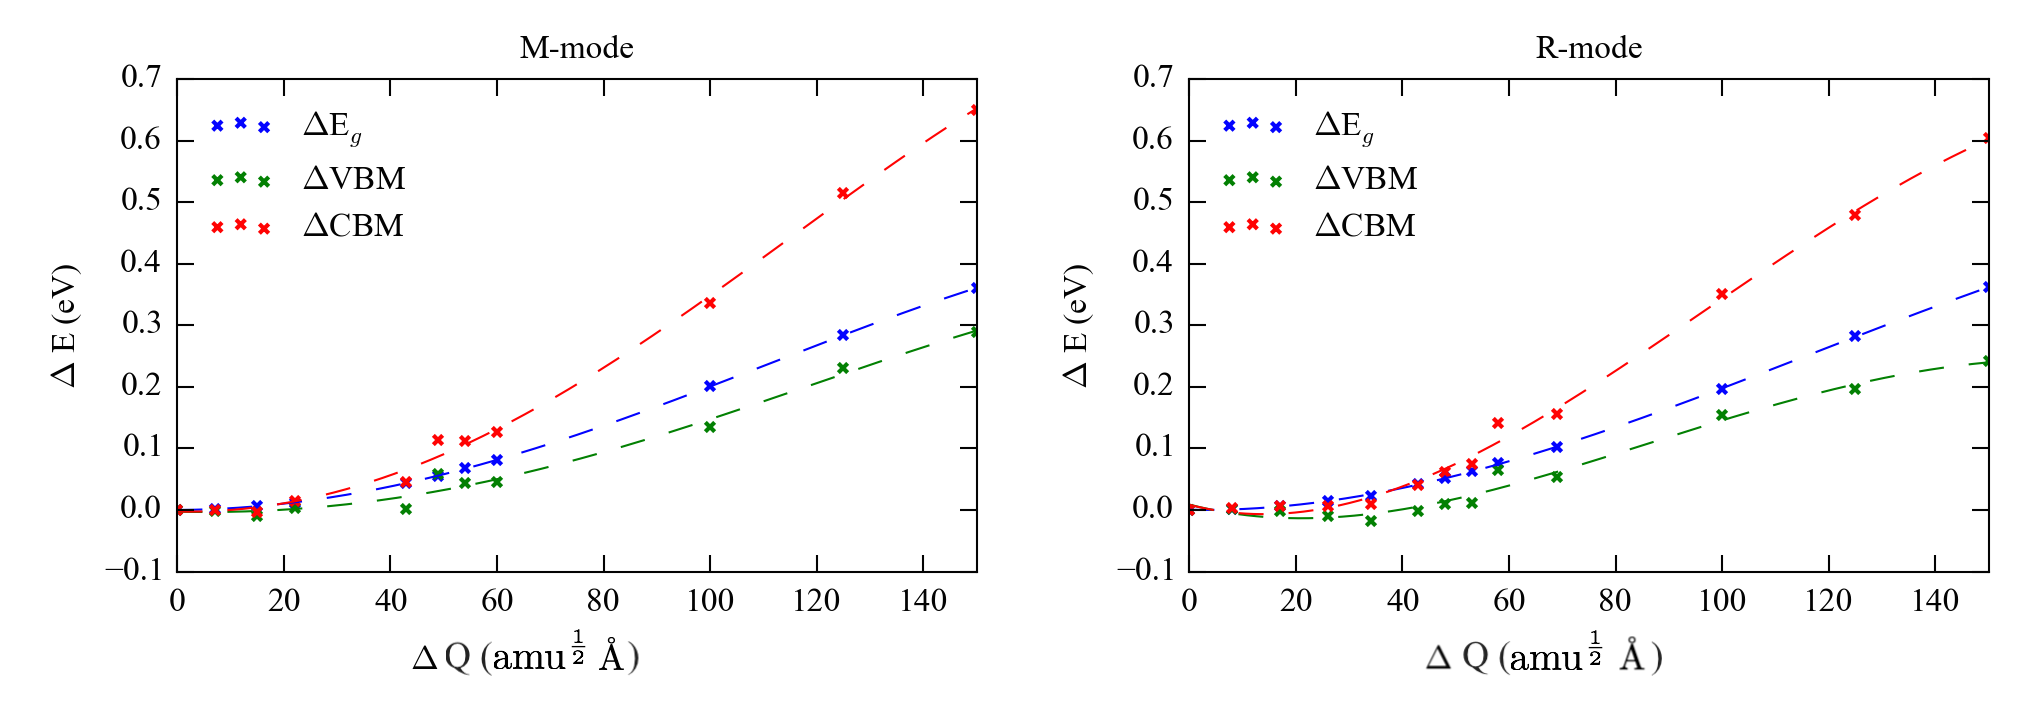
\includegraphics[width=\textwidth]{figures/ch5/fig_s3.png} \label{ch5figs1}
\caption[Bandgap deformation potential]{
Energy change ($\Delta$E) as a function of the normal-mode coordinate $Q$ of the valence-band maximum ($\Delta$VBM), conduction-band minimum ($\Delta$CBM), and band gap ($\Delta$E$_g$) obtained from calculations using the PBEsol functional.
The energies of the band extrema have been referenced to the energy of the Pb 3d core states.
}
\end{figure}


\begin{table}[ht] \label{ch5rsstable}
 \caption[Residual sum of squares for quadratic and bi-quadratic fits to calculated bandgaps] {Residual sums of squares (RSS) for quadratic and biquadratic fits to the data in Fig. \ref{ch5figs1}. A smaller RSS indicates a better fit of the model to the data.}
  \label{RSS} 
 \begin{tabular}{cccc} 
 \hline  \hline
 
  \multicolumn{1}{c}{} & $\Delta$VBM & $\Delta$CBM & $\Delta$E$_g$ \\
  \hline
 \multicolumn{1}{c}{} & \multicolumn{3}{c}{$M$} \\

 Quadratic & $4.1 \times 10^{-3}$ & $ 1.1 \times 10^{-2}$ & $3.7 \times 10^{-3}$ \\

 Biquadratic & $3.2 \times 10^{-3}$ & $2.9 \times 10^{-3}$ & $2.0 \times 10^{-5}$ \\

 \hline 
 
  \multicolumn{1}{c}{} & \multicolumn{3}{c}{$R$} \\

 Quadratic &   $9.8 \times 10^{-3}$& $2.0 \times 10^{-2}$& $3.5 \times 10^{-3}$\\

 Biquadratic & $6.4 \times 10^{-3}$ &$6.0 \times 10^{-3}$ & $6.0 \times 10^{-5}$\\
 
 \hline \hline
 \end{tabular}
 \end{table}

\begin{table}[h] \label{ch5abtable}
\caption[Bi-quadratic fit coefficients at three levels of theory] {Values of the $a$ and $b$ coefficients in the fitted function $E_g = E_0 + aQ^2 + bQ^4 + O(Q^6)$ used to model the band gap deformation potentials evaluated from frozen-phonon calculations using the PBEsol, PBEsol+SoC and HSE06 exchange-correlation functionals.}
\label{bandgapF}
\begin{tabular}{ccccccccc} 
    \hline\hline
{Mode} & \hspace{5pt} & {} & \hspace{5pt} & {PBEsol} & \hspace{5pt} & {PBEsol+SoC}& \hspace{5pt} & {HSE06}\\ 
    \hline
$M$ && $a$ && \num{2.3e-5}     && \num{2.3e-5}       && \num{2.9e-5} \\
    && $b$ && \num{-3.3e-10}   && \num{-3.6e-10}     && \num{-5.4e-10} \\
$R$ && $a$ && \num{2.3e-5}     && \num{2.5e-5}       && \num{2.9e-5} \\
    && $b$ && \num{-3.0e-10}   && \num{-4.3e-10}     && \num{-7.0e-10} \\ 
    \hline\hline
\end{tabular}
\end{table}



\subsubsection{Exchange-correlation functional and spin dependence}

Our tests on two different descriptions of electron exchange and correlation and one including spin-orbit coupling, shows similar behaviour with respect to band deformation (Table \ref{Egtheory} and Figure \ref{ch5allxc}). 
 % the distortion for hybrid is more: increased localisation couples more strongly to lattice distortions?
 
\begin{figure}[]
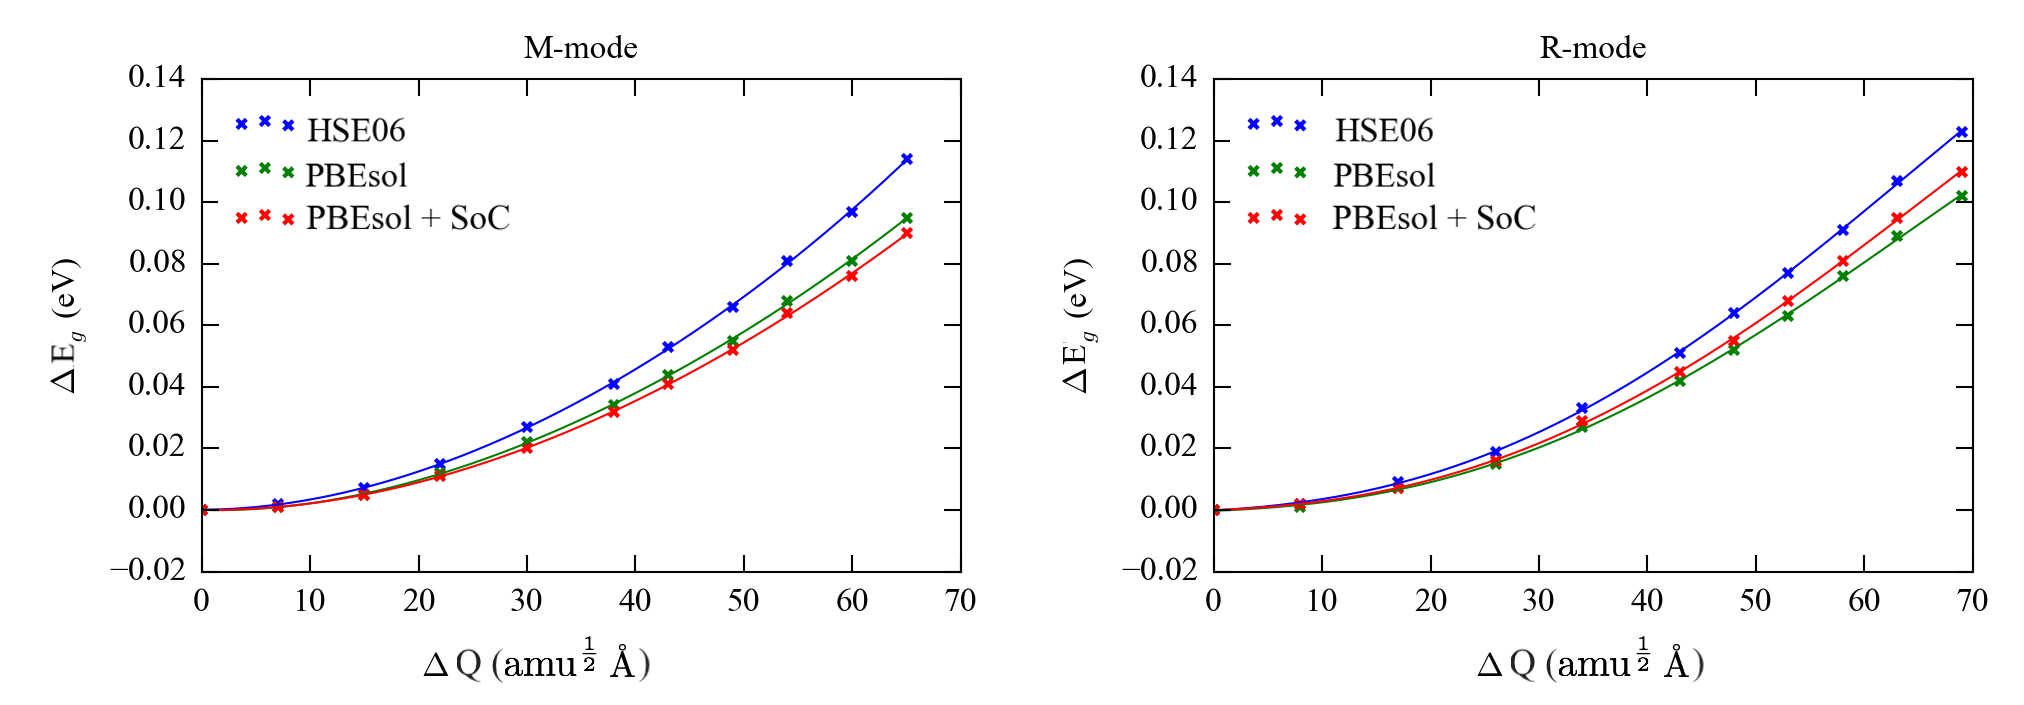
\includegraphics[width=\textwidth]{figures/ch5/fig_s4.png} \label{Egtheory}
\caption[Bandgap deformation at three levels of theory]{
Change in band gap ($\Delta E_g$) as a function of the normal-mode coordinate $Q$ obtained with three exchange-correlation treatments used in the electronic-structure calculations, \textit{viz.} PBEsol, PBEsol with spin-orbit coupling (SoC), and HSE06.
}
\end{figure}

\begin{table}[]
\caption[Valence- and conduction-band deformation potentials]{
Valence- and conduction-band deformation potentials relative to the Pb 3d core energy level obtained from frozen-phonon calculations with three exchange-correlation treatments, \textit{viz.} PBEsol, PBEsol with spin-orbit coupling (SoC), and HSE06.
}
\begin{tabular}{ccccccccc} \label{ch5allxc}
Mode & \hspace{5pt} & & \hspace{5pt} & PBEsol & \hspace{5pt} & PBEsol+SoC & \hspace{5pt} & HSE06 \\
$M$ & & VBM & & $1.61 \times 10^{-5}$ & & $1.55 \times 10^{-5}$ & & $0.97 \times 10^{-5}$ \\
& & CBM & & $3.88 \times 10^{-5}$ & & $3.68 \times 10^{-5}$ & & $3.66 \times 10^{-5}$ \\ 
& & $\frac{CBM}{VBM}$ & & 2.14 &  & 2.37 & & 3.77  \vspace{5pt} \\

$R$ & & VBM & & $1.34 \times 10^{-5}$ & & $1.01 \times 10^{-5}$ & & $1.33 \times 10^{-5}$ \\
& & CBM & & $3.52 \times 10^{-5}$ & & $3.37 \times 10^{-5}$ & & $3.96 \times 10^{-5}$ \\
& & $\frac{CBM}{VBM}$ & & 2.63 & & 3.34 & & 2.98 \vspace{5pt} \\ 
\end{tabular}
\end{table}

% check how these deformation potentials have been calculated.

\subsection{Temperature dependant bandgap broadening} \label{ch5coupling}

Distortions along the $M$ and $R$ phonon modes produce the familiar double-well potential energy surface as shown in the literature review, Figure \ref{}
The undistorted high-symmetry cubic perovskite structure is a saddle point between two equivalent broken-symmetry solutions. The barriers are 37meV and 19 meV for the $R$ and $M$ modes respectively, which is comparable to $K_BT$, and dynamic disorder is expected.
The Schr ̈odinger equation describing nuclear motion in the potential energy surfacein  Figure \ref{} can be solved following a procedure outlined in Ref. [].\cite{}% jonathan paper: https://journals.aps.org/prl/pdf/10.1103/PhysRevLett.117.075502 \cite{} JArv's code.

The average bandgap as a function of temperature $E_g(T)$ can then be calculated from the thermally populated vibrational eigenstates $\chi(Q,T)$ that form a solution to the 1D schrodinger equation:
\begin{equation}
E_g(T) = \langle \chi(Q,T)|E_g(Q)|\chi(Q,T) \rangle
\end{equation}

Using this procedure, there is a positive band-gap shift of 35.5 meV (Rmode) and 27.9 meV (Mmode) at T=300 K, which is comparable in magnitude to the measured broadening of 40 meV [41]. 
% And a note about the significance of this result?? Is it large??

\subsubsection{A note on supercell size}

The cartesian displacement of atoms in a $N_a$ atom unit cell for a phonon mode with amplitude $Q$ scales as $\frac{Q}{\sqrt{N_a}}$.\cite{}%link to phonopy documentation here
The bandgap deformation is a function of cartesian displacement, so that doubling the size of the supercell will scale the atomic displacements and bandgap change by a factor of $\frac{1}{\sqrt{2}}$ (Figure \ref{ch5scaling}).  % I don't really understand this!
Importantly, changing the supercell size scales the x-axis of the mode potential in the Schrodinger solver so that the average band gap for a given temperature, a physical observable, does not scale with supercell size.

\begin{figure}[]
\includegraphics[width=\textwidth]{figures/ch5/fig_scaling.png} \label{ch5scaling}
\caption[Bandgap deformation and supercell size]{
Change in bandgap and the potential energy surface for two supercell sizes.  To allowfor comparison thex-axis values for the 2×2×1 supercell have been scaled to match those of the2×2×2 supercell and the potential energy of the 2×2×1 supercell has been doubled.  Differencesin the calculated bandgap are of the order 10−4eV.
}
\end{figure}

\subsection{Hot carrier cooling mechanisms}
In the previous section we considered how the electronic sub-system couples to the vibrational sub-system. We considered distortion along a single phonon mode and neglected coupling between phonon modes. In this section we consider the interaction between phonon modes.

\subsubsection{Polaron formation}
The Frohlich polaron model was recently applied to MAPI.\cite{} %Jarvist
When the polaron coupling is weak the kinetic energy is larger than the polaron binding energy, the polaron radius is larger than a unit cell - a large polaron is formed. When the polaron coupling is strong the electron is self-trapped, the polaron radius is the size of a unit cell or smaller - a small polaron is formed. The calculated Fro ̈hlich coupling constants are $\alpha=2.4$ and $\alpha=2.7$ for the electron and hole respectively. These values fall in the intermediate coupling regime where the large polaron model is valid.  The solution to Frolich model in Ref. [] gives a polaron radii of $26.8\AA$ and $25.3\AA$ for the electron and hole respectively, at 300K.

The calculated polaron radius is an upper bound: bulk polaron states are further localised by disorder, point defects and extended defects such as surfaces, interfaces and grain boundaries.


\subsubsection{Initial thermalisation}
After polaron formation there is initial thermalisation, where electron kinetic energy is transferred into the optical phonon modes. This is a fast picosecond process via the strong Frolich coupling between the charge carrier and localised, polar phonon population.
Once fully thermalised, the above bandgap energy is distributed amongst all phonon states associated with the polaron.

The temperature of the resulting Fr{\:o}lich polaron depends on the polaron volume, the polaron specific heat capacity $c_v$ and the initial excitation energy (Figure \ref{ch5TemperatureRadius}). We assume that the initial excitation energy is distributed evenly between the electron and hole. The heat capacity is calculated from the bulk phonon density of states: summing over the Bose-Einstein occupied phonon modes for MAPI, the per-unit cell specific heat capacity is \SI{1.25}{\milli\eV\per\K} at
\SI{300}{\K}. Near-UV excitation at 4eV gives a maximum energy of 1.2eV which can be transferred to the polaron, and the temperature increases with localisation ($T \propto r^{-3}$).

\begin{figure}[h]
\centering
  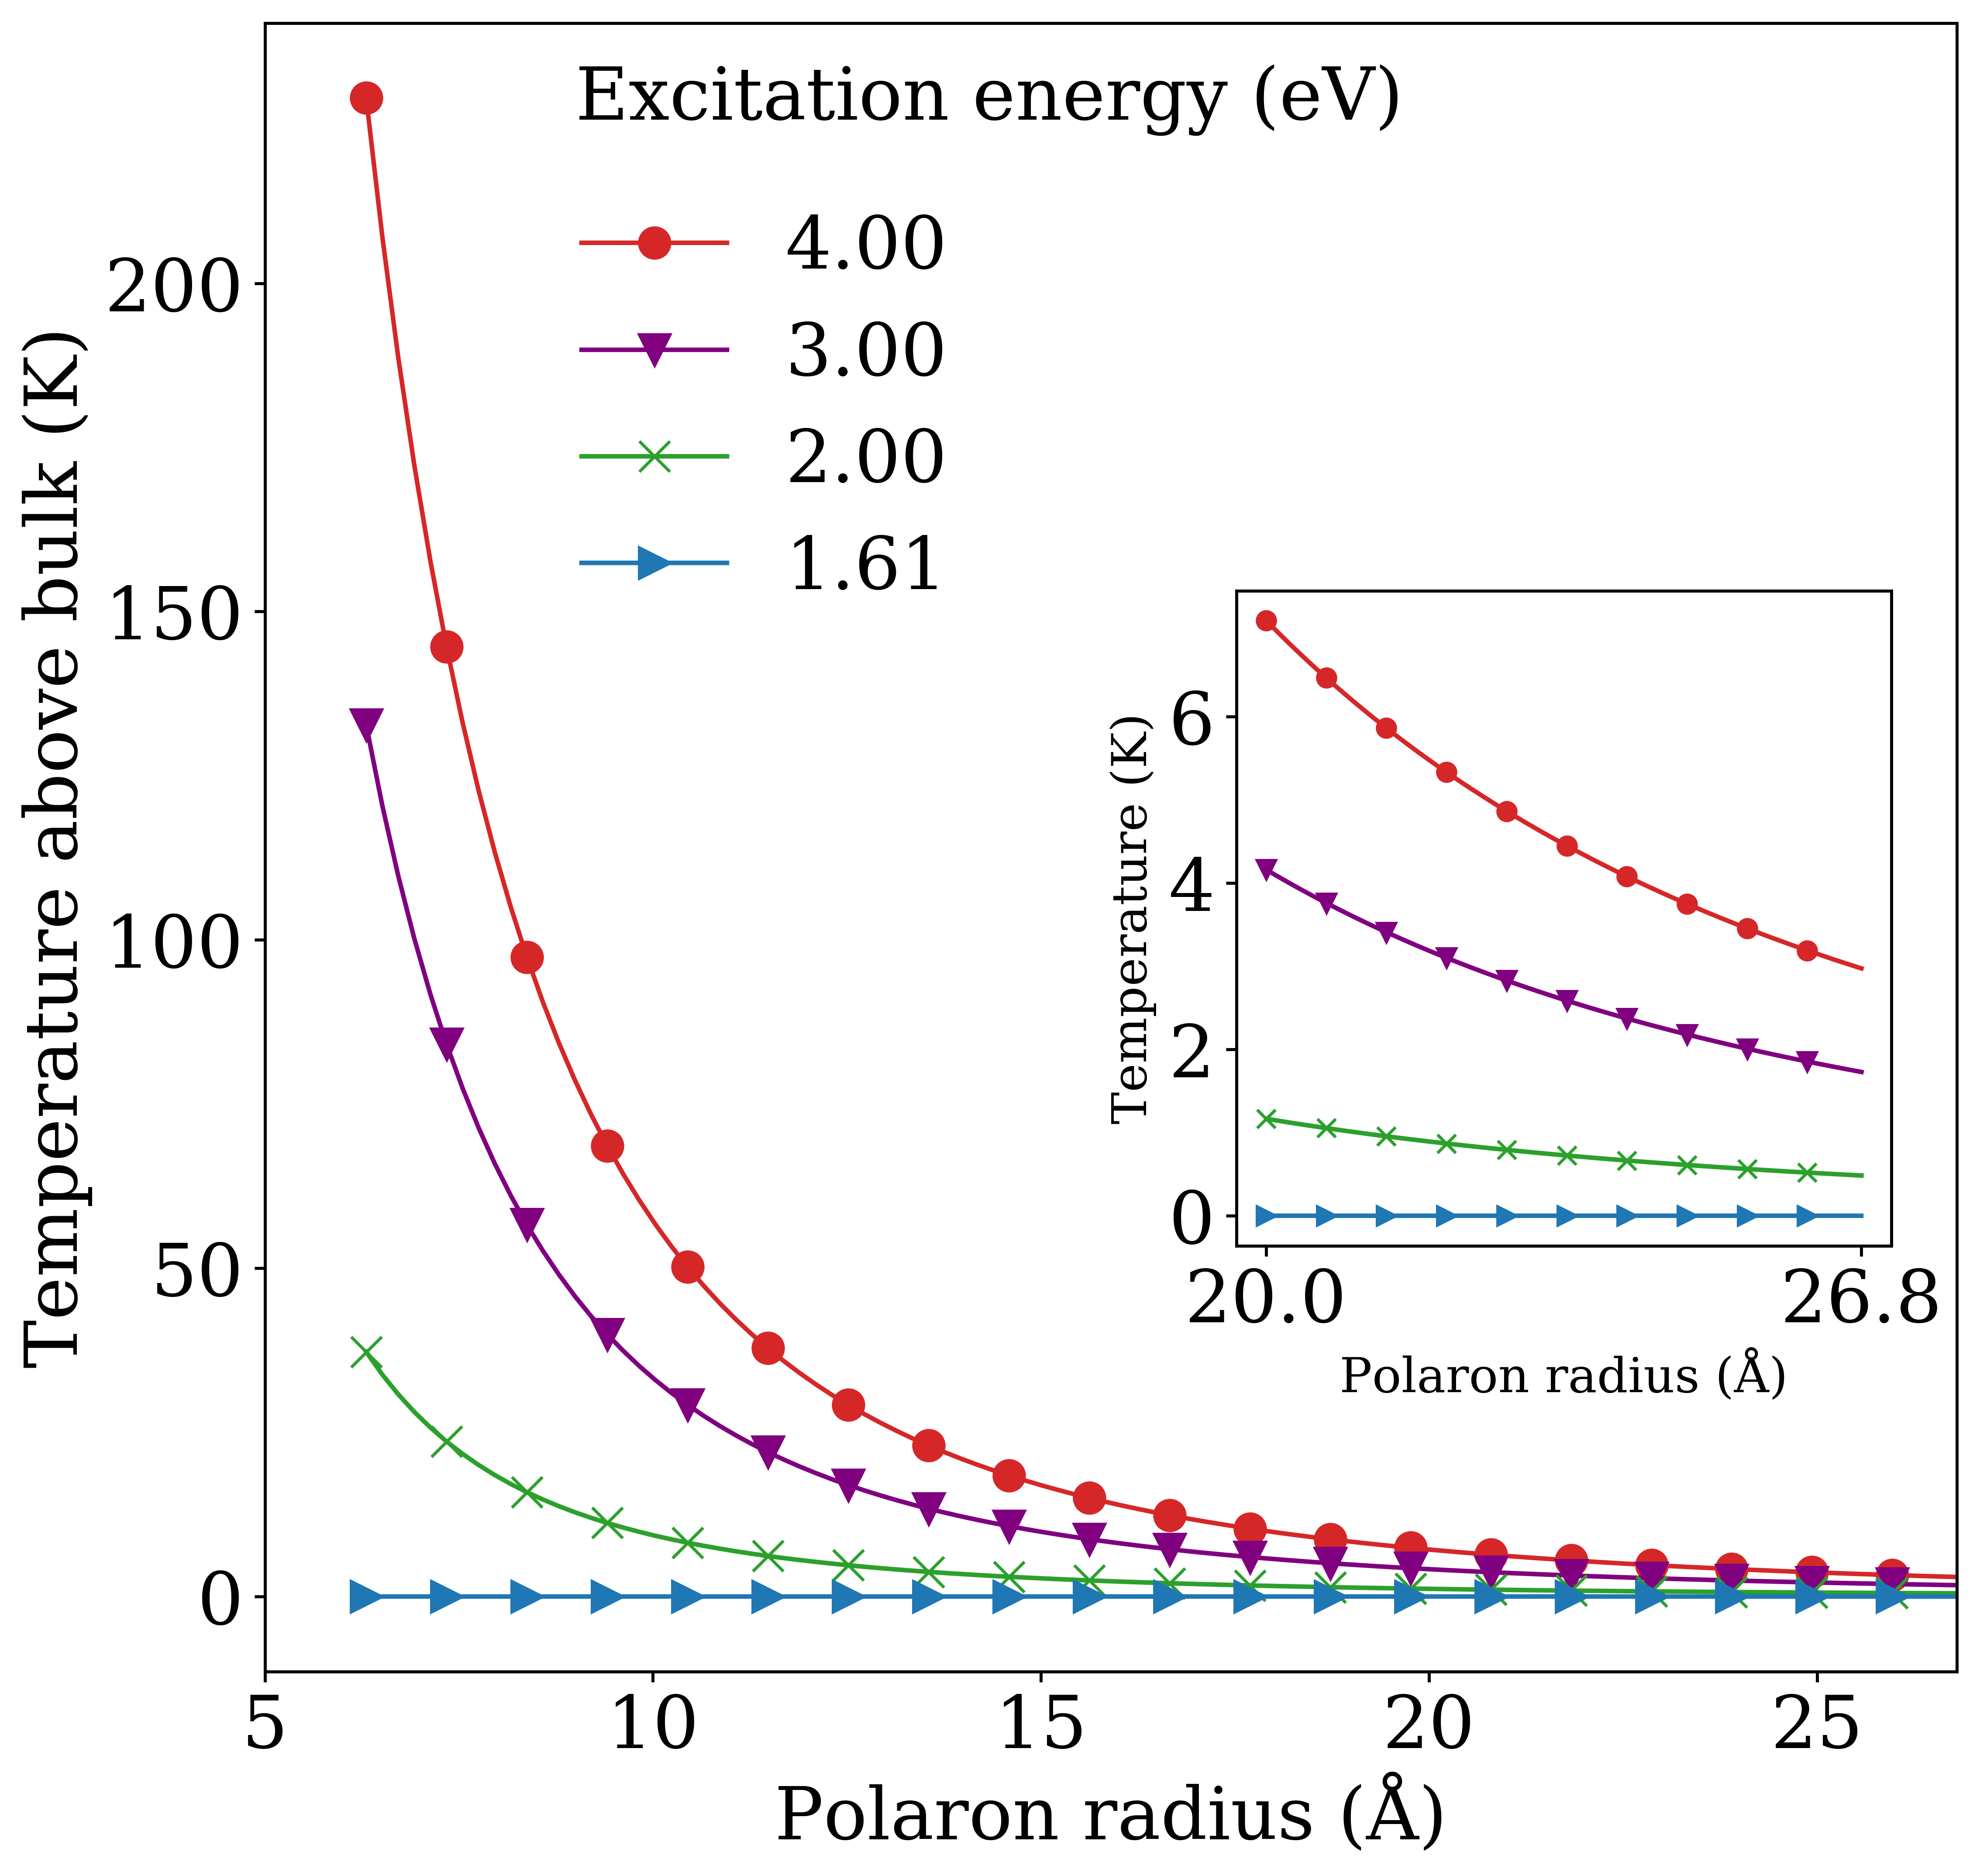
\includegraphics[width=1\textwidth]{figures/ch5/f3.png}
  \caption[Polaron temperature as a function of polaron radius]{Thermalised polaron temperature in MAPI as a function of polaron
    radius and excitation  energy assuming a bulk value of the heat capacity. 
    The calculated bulk electron polaron radius
    of 26.8 \AA provides an upper bound for polaron size.
    We take the lattice parameter (6.3 \AA) as a lower bound---below this the
    continuum large polaron approach is not valid. 
    We consider excitation from the bandgap to near-UV. 
    Inset shows detail at larger radii (axes same as main). }
  \label{ch5TemperatureRadius}
\end{figure}

% how we calculate teh specific heat. The theory has been outlined clearly by Jarvist Frost, and Independantly verified by myself.

\subsubsection{Cooling to equilibrium}
After a fast initial thermalisation, the polaron will cool to equilibrium over a longer timeframe. During this cooling process the excited local optical phonon modes scatter into phonon modes that diffuse away from the polaron.

Due to energy and momentum conservation rules, three-phonon scattering is the lowest-order scattering process.  The three-phonon interaction strengths have been calculated for MAPI, \cite{} and they are found to be orders of magnitude stronger than for CdTe and GaAs. The strong three-phonon interactions strengths produce a bulk thermal conductivity, calculated from a solution of the Boltzmann transport equation in the relaxation time approximation, that is extremely low; \SI{0.05}{\watt\per\metre\per\K} at \SI{300}{\K}.\cite{Whalley2016} 
In contrast, the calculated conductivity for GaAs and CdTe is 
\SI{38}{\watt\per\metre\per\K}
and
\SI{9}{\watt\per\metre\per\K},
respectively.

\begin{figure}[h]
\centering
  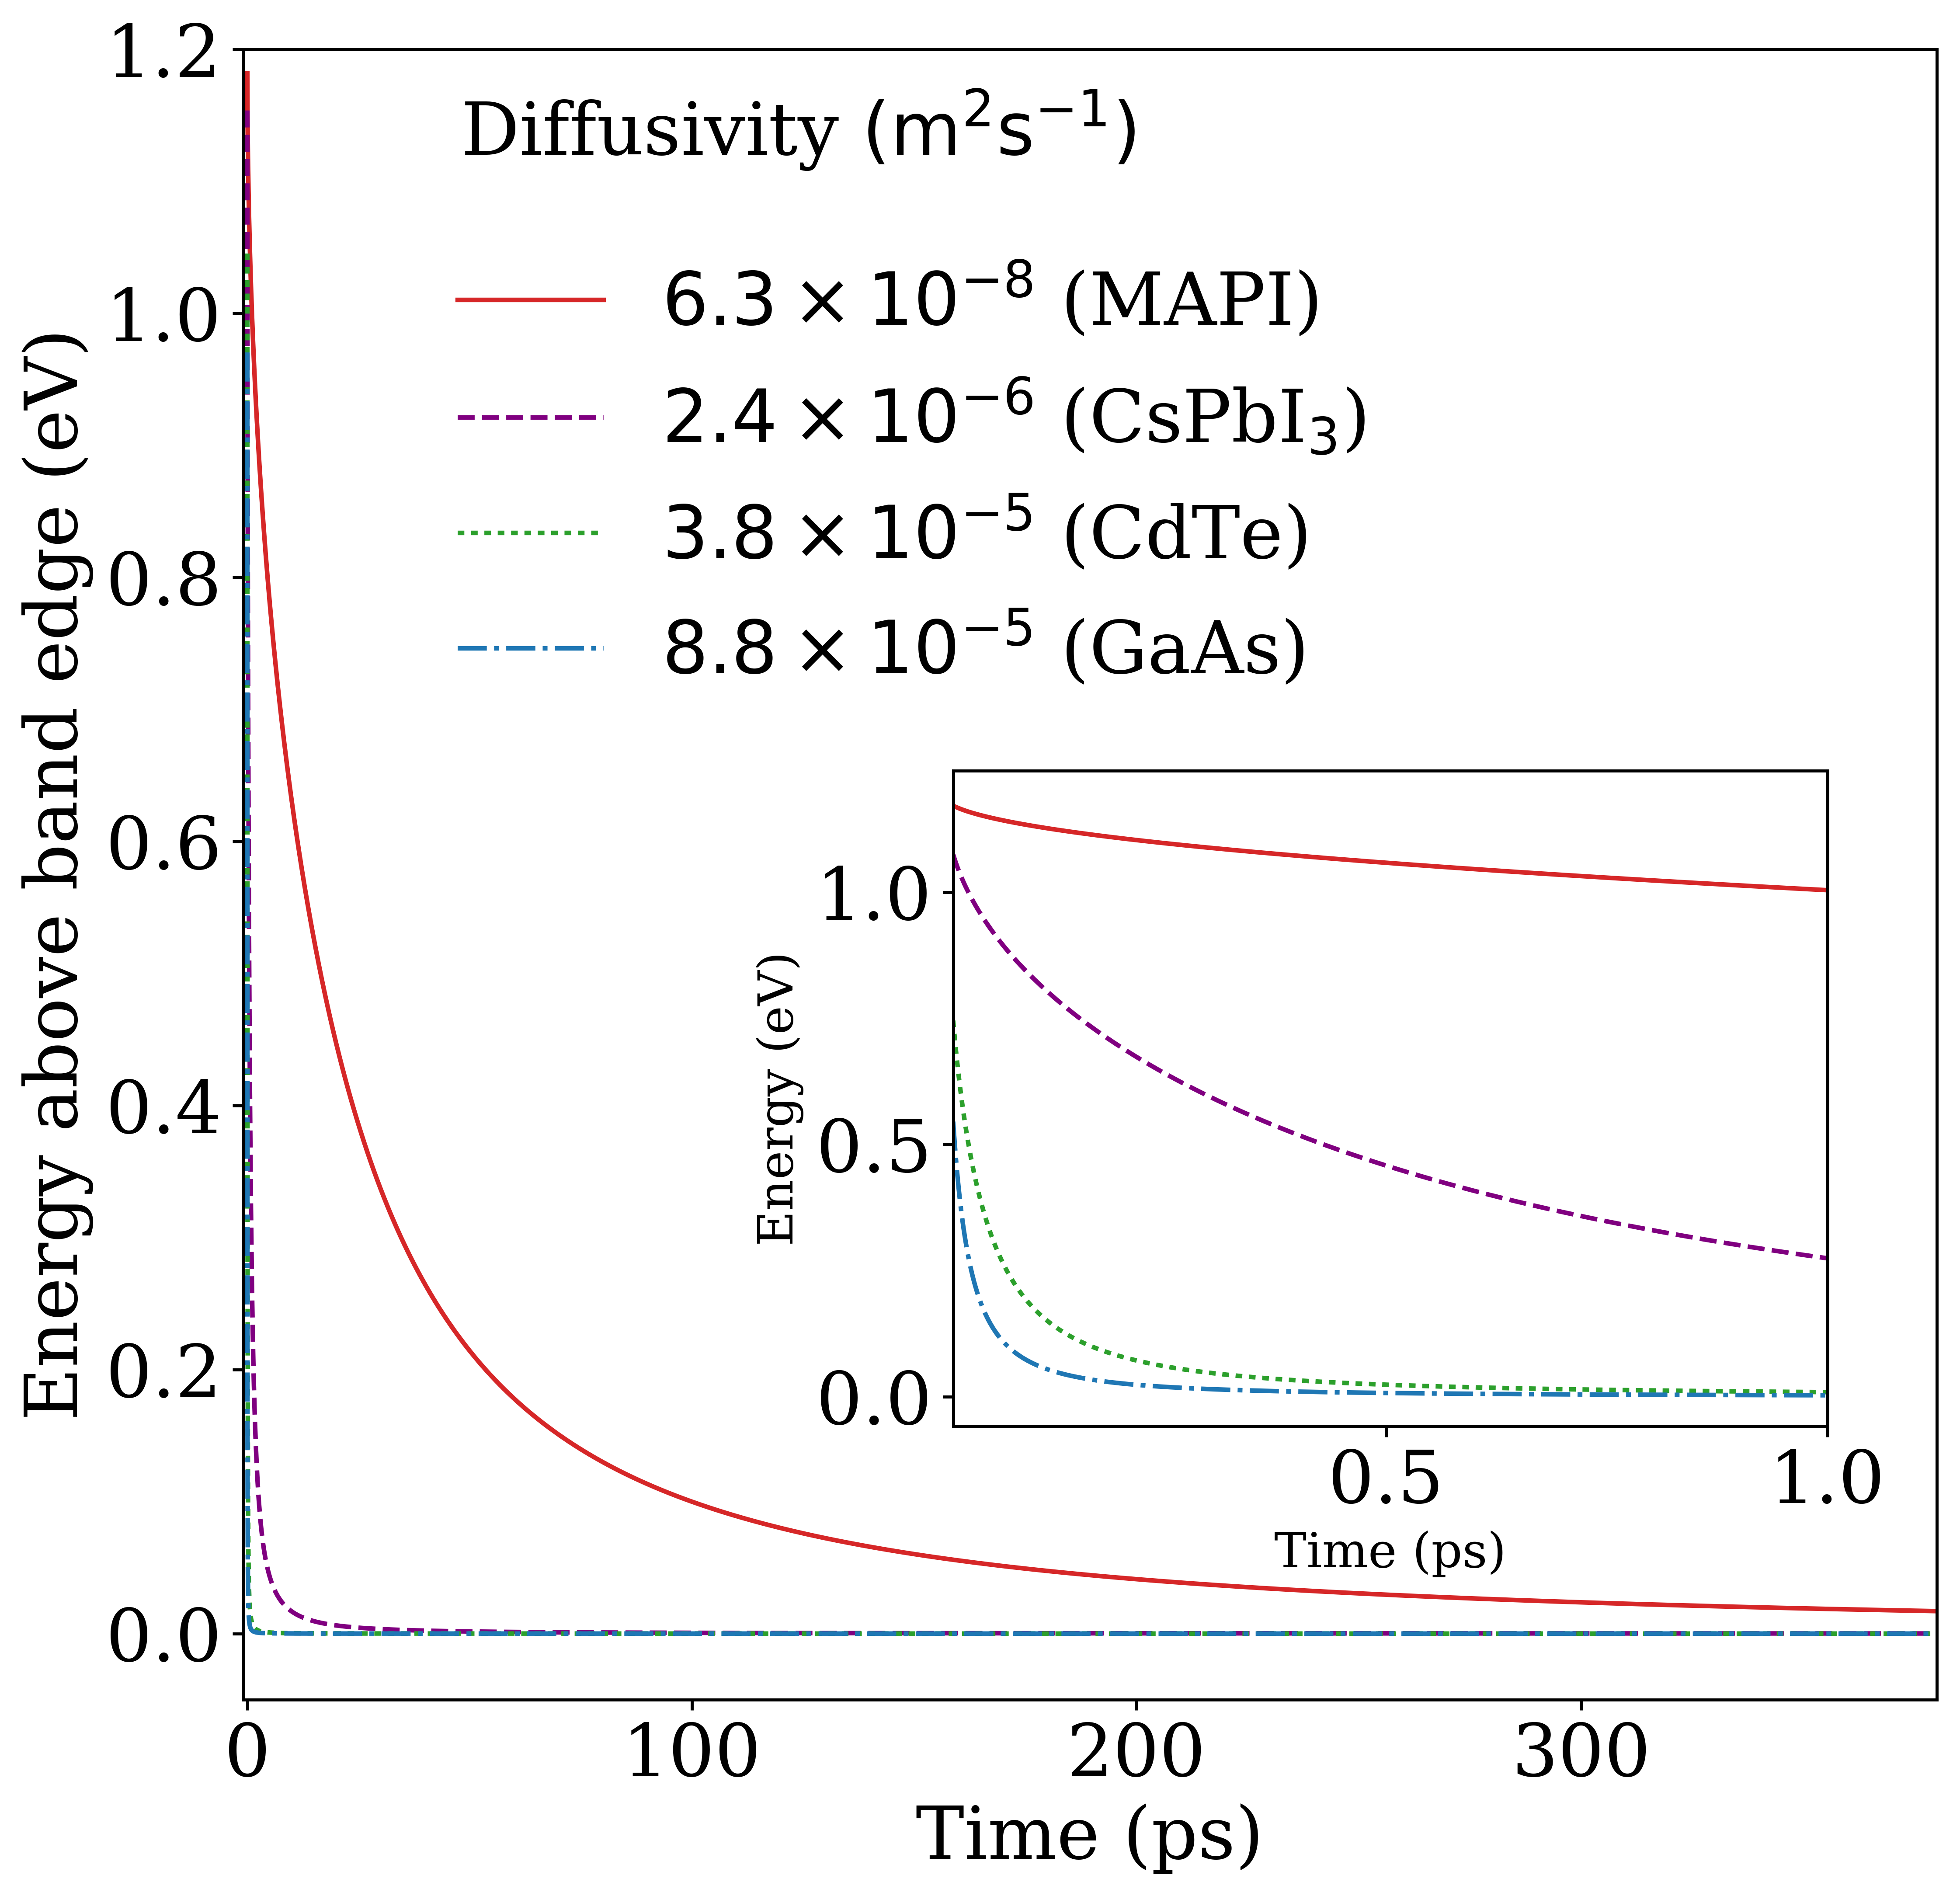
\includegraphics[width=1.0\textwidth]{figures/ch5/f4.png}
  \caption[Hot carrier cooling rate]{The energy of a large polaron state (starting at 1.2 eV above the conduction band minimum, with a polaron radius of 26.8 \AA) 
  in \ce{CH3NH3PbI3} as a function of time.
  The slow rate is due to the low thermal conductivity in MAPI ($\kappa$ = 0.05Wm$^{-1}$K$^{-1}$). 
  For comparison, we show the behaviour using the thermal conductivities of 
  CdTe ($\kappa$ = 9) and GaAs ($\kappa$ = 38). }
  \label{ch5TemperatureTime}
\end{figure}

To model the third order phonon-phonon scattering processes we consider the polaron as a hot sphere in a continuum of ambient temperature material, which allows us to calculate temperature as a function of time using the heat diffusion equation.
We consider the low fluence limit where individual photon quanta are absorbed into isolated hot polarons.
The rate of cooling is determined by the diffusivity ($D$): 
\begin{equation}
    D= \frac{\kappa}{\rho c_p}
\end{equation} 
where $\kappa$ is the thermal conductivity, $\rho$ is the density and $c_p$ is the specific heat capacity. 

Heat diffuses from MAPI on the order of 100 ps, whilst for other conductivities the process is much faster, on the order of 100 fs. 
This is in agreement with reported experimental values: Refs. \cite{Klein2016} (MAPI), \cite{Zhong2017} (CdTe) and \cite{Rosenwaks1993} (GaAs). 
Note that at short timescales, measurements of hot carrier cooling in MAPI and \ce{CsPbI3}($\kappa$ = 0.5) may appear linear due to the slower exponential decay.

\section{Summary}

We have shown how Fr{\:o}lich polaron theory and a classical heat diffusion model can be combined to
describe the physical process behind the slow hot-carrier cooling rates
observed for halide perovskites.
In the previous section we assumed athermal, that temperature played no role. In this chapter we have "turned on" temperature and outlined two consequences; electron-phonon and phonon-phonon.

\textbf{Data Access Statement}\\
The crystal structures and phonon data are available at \url{https://github.com/WMD-group/Phonons}. 
and can be processed using the \textsc{Phonopy} packages available from \url{http://atztogo.github.io/phonopy} 

Data files and Jupyter notebooks outlining the calculation steps are available as a repository on GitHub at https://github.com/WMD-group/hot-carrier-cooling.
\textbf{Acknowledgements}\\
Via our membership of the UK's HEC Materials Chemistry Consortium, which is funded by EPSRC (EP/L000202), this work used the ARCHER UK National Supercomputing Service (http://www.archer.ac.uk).
Calculations were performed on the SiSu supercomputer at the IT Center for Science (CSC), Finland, via the Partnership for Advanced Computing in Europe (PRACE) project no. 13DECI0317/IsoSwitch. We also made use of the Balena HPC facility at the University of Bath, which is maintained by Bath University Computing Services.


